
\section{Luck}
\lucasc{@Ian, this is something from the forum on the kaggle comp, it is answering a question about scoring predictions. }
\ianc{What's this guy talking about?}
\noindent It's not about the prize, it's the element of luck involved...\\
\noindent  William Cukierski, Kaggle Competition Admin \\

Previously, we detailed popular methods for prediction and outlined our new methodology that accounts for specific match ups. In this section of this paper, we address the high degree of chance present in NCAA tournaments and consequently prediction for NCAA tournaments.  Specifically, we address sensitivity of a Kaggle style leader board. While it is natural to think 2nd place almost won, we aim to answer the question how close was 20th place to winning? 

% some verbiage in here... 

To study the effect of luck we take the idea that the 2nd place team almost won and we attempt to quantify `almost.' To this end, we examine alternate realities where a losing team in an overtime game is treated instead as a winning team. We focus only on overtime games because it seems most reasonable to think of the losing team as having won in those cases. Recall that the loss function used for scoring of the Kaggle competition is

\lucasc{Maybe we can omit this equation if it is defined in an earlier section and just number that version and refer to that equation number here?} 
\begin{equation}\label{eqn:kaggle_score}
-\sum_{i=1}^n\frac{y_ilog(p_i)+ (1-y_i)log(1-p_i)}{n},
\end{equation}
where $y_i$ is a binary variable taking value 1 when the team wins and 0 otherwise and $0 \leq p_i \leq 1$ denotes the predicted value for the team in the $i$th game. We consider how dependent the rankings of individual teams are on the characteristics of the particular loss function. To answer this question we studied a couple of possible alternate scoring functions. We consider the following scoring functions: 
 
\begin{equation}\label{eqn:first_score_function}
-log(1-2|.5-p_i|)
\end{equation} 

\begin{equation}\label{eqn:second_score_function}
-log(1-|.5-p_i|)
\end{equation} 

\begin{equation}\label{eqn:third_score_function}
-log(1-|y_i-p_i|)
\end{equation} 
Here, for brevity, we only write the part of the loss function multiplied by the $(1-y_i)$ term. Moreover, in Function \ref{eqn:third_score_function}, $y_i \in \{0,.5,1\}$, where now the $0.5$ is the realized value when teams go into overtime, the other equations use only $y_i \in \{0,1\}$. Figure \ref{fig:scoring_functions} is a plot of the different score functions for values $0\leq p_i \leq 1$.  

\ianc{It's not clear how these functions correspond to the lines in the plot below. We're also not sure that it's necessary to consider so many marginally different loss functions.}

\begin{figure}[H]
\centering
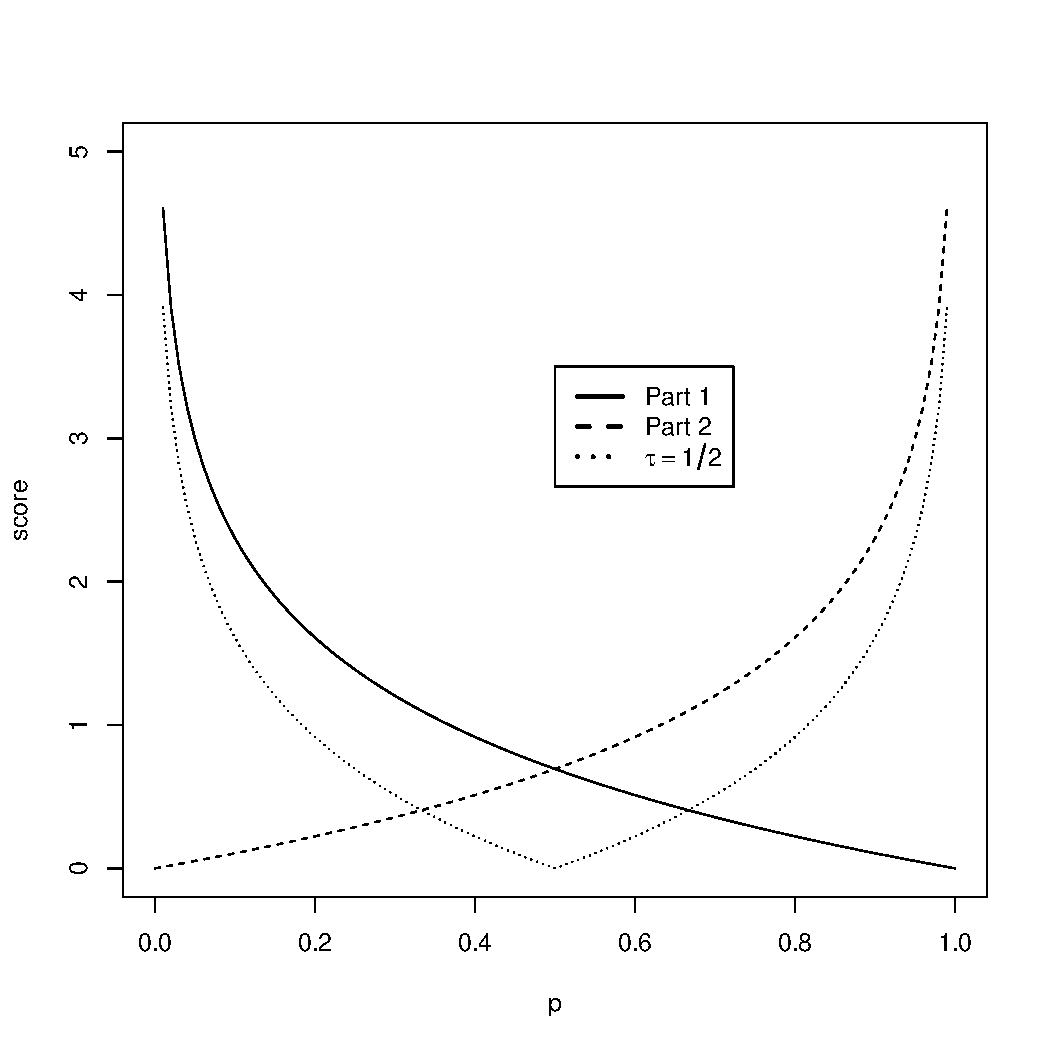
\includegraphics[width=.7\textwidth]{loss_function_plot_bw.pdf}
\caption{A plot of the various loss functions as a function of the prediction $p_i$.  }
\label{fig:scoring_functions}
\end{figure}

It is clear from looking at Figure \ref{fig:scoring_functions} that the different scoring functions treat the contestant's confidence differently. Both Equations \ref{eqn:first_score_function} and \ref{eqn:second_score_function} are symmetric about 0.5, which is aesthetically pleasing and a useful attribute for handling tied or overtime games in a slightly different manner than games with a clear victor. Moreover, Equation \ref{eqn:first_score_function} penalizes much more for confident predictions than Equation \ref{eqn:second_score_function}. 

One might wonder, given the plethora of choices one might use to rank contestants, how much is a result of a specific scoring function and how much much change of  we moved from one scoring function to another? To examine this, we made a plot of the contestant predictions scored under the various loss functions described above. The results of this plot are shown in Figure \ref{fig:score_rank_plot}. 

  \begin{figure}[h]
\centering
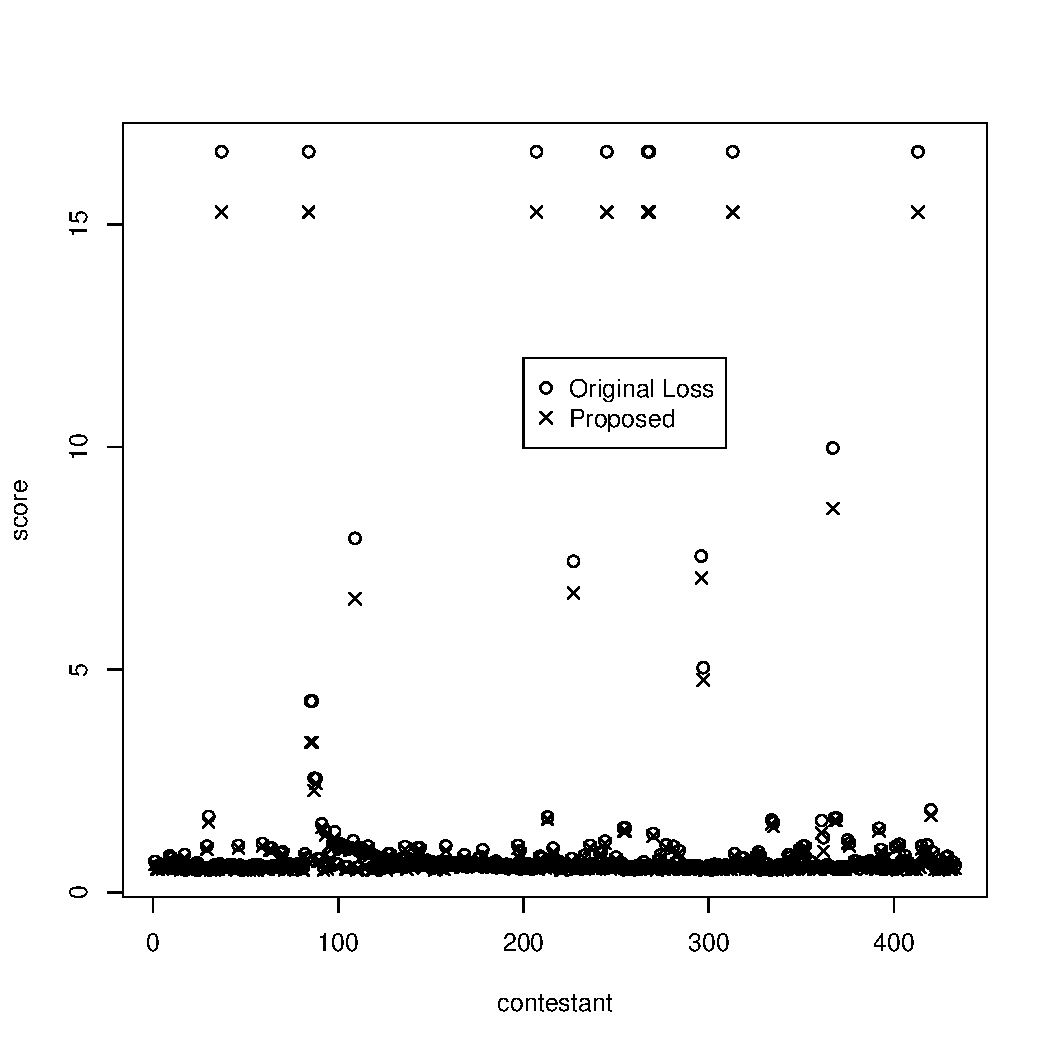
\includegraphics[width=.7\textwidth]{prelim_rank_plot1_bw.pdf}
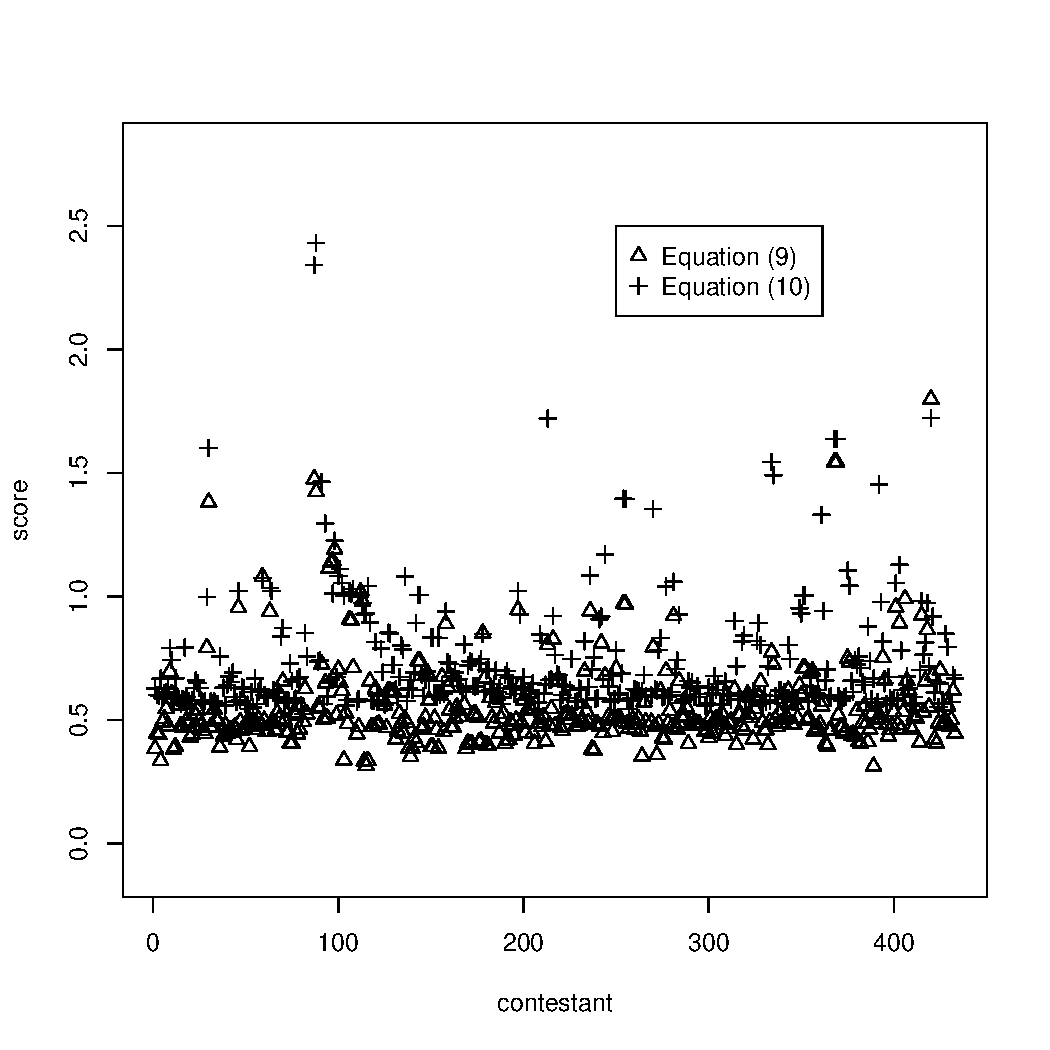
\includegraphics[width=.7\textwidth]{prelim_rank_plot2_bw.pdf}

\caption{The scores of each contestant under the different loss functions. A smaller score is better.  }
\label{fig:score_rank_plot}
\end{figure}

Given that the choice of scoring function can affect the contestants' positions on the leaderboard, we did a correlation analysis of the contestant submissions resulting from the actual scoring function, Equation \ref{eqn:kaggle_score} and correlated these ranks against the ranks of the contestants under the other three scoring functions. The results of this analysis are shown in Table \ref{tab:kendall_tau_table} beneath. There appear to be little correlation between the resultant rankings, indeed, there was not a single significant p-value amongst the results.  Of course one might think, there can be little overall correlation between the rankings but still the top three might be the same or similar across the various scoring functions but this turned out not to be the case. In fact, comparing the top three on the leaderboards for the different scoring functions show no common contestants. Additionally, we looked at the three worst contestants as well, here the trend was the same, no common contestants when scoring using different criteria. 

\begin{table}[ht]
\centering
\begin{tabular}{rrr}
  \hline
Score comparison & $\tau$ & p-value \\ 
  \hline
\ref{eqn:kaggle_score} vs. \ref{eqn:first_score_function} & -0.00 & 0.97 \\ 
\ref{eqn:kaggle_score} vs. \ref{eqn:second_score_function} & 0.01 & 0.79 \\ 
\ref{eqn:kaggle_score} vs. \ref{eqn:third_score_function} & 0.05 & 0.09 \\ 
\ref{eqn:first_score_function} vs. \ref{eqn:second_score_function} & -0.03 & 0.42 \\ 
\ref{eqn:first_score_function} vs. \ref{eqn:third_score_function}   & -0.05 & 0.15 \\ 
\ref{eqn:second_score_function} vs. \ref{eqn:third_score_function}  & 0.00 & 0.96 \\ 
   \hline
\end{tabular}
\label{tab:kendall_tau_table}
\caption{}
\end{table}



Leakage is defined by \cite{schutt2013doing} as an accidental inclusion of `future' data into the training set. \cite{schutt2013doing} state that in earlier days of online comptitions they were able to consistently win competitions by systematically exploiting leakage. While much has been made in contest forums and in books  about leakage and how leakage is often exploited to win competitions, it is somewhat refreshing to see that other choices like the scoring function play into the relative results of a competition. While leakage might be the result of competition administrators' errors, or a misunderstanding of the data generating process, the scoring function should be chosen to match the reality of the errors made while forecasting. While luck ultimately plays a role in the basketball games themselves and the results of prediction tournaments, some players are able to consistently outperform. While this section has depicted alternate outcomes that could have occurred, an actual alternate outcome will not arise until next year when the tournament occurs.  These consistent outperformers are lucky, but lucky in the sense that they managed to get the right results for their specific loss function used in the competition. The results shown here indicate that if a contestant does not explicitly incorporate the loss function into their predictions, they are leaving their winnings more to chance than to skill. 